\documentclass[tikz]{standalone}

\usepackage{amsmath}
\usepackage{physics}

\usetikzlibrary{arrows.meta,fit,positioning}

\begin{document}
	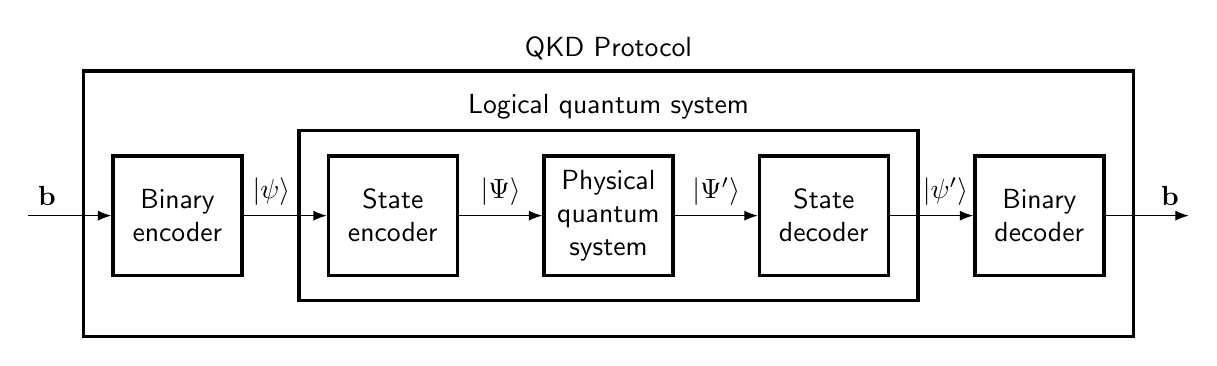
\begin{tikzpicture}[
		node distance=3em,
		block/.style={draw, very thick, minimum height=10ex, minimum width=3.5em, text width=4em, align=center},
	]
		\node[block] (phy) {\textsf{Physical quantum system}};
		\node[block, left=of phy] (senc) {\textsf{State encoder}};
		\node[block, right=of phy] (sdec) {\textsf{State decoder}};
		\node[block, fit=(senc) (sdec), inner xsep=1em, inner ysep=2ex, label={\textsf{Logical quantum system}}] (log){};
		\node[block, left=of senc] (benc) {\textsf{Binary encoder}};
		\node[block, right=of sdec] (bdec) {\textsf{Binary decoder}};
		\node[block, fit=(benc) (bdec), label={\textsf{QKD Protocol}}, inner xsep=1em, inner ysep=6ex, yshift=1ex] (proto) {};

		\coordinate[left=of benc] (in);
		\coordinate[right=of bdec] (out);
		
		\draw[-Latex] (in) node[above right]{$\vb{b}$} -- (benc);
		\draw[-Latex] (benc) -- (senc) node[midway, above, xshift=-0.5em]{$\ket{\psi}$};
		\draw[-Latex] (senc) -- (phy) node[midway, above]{$\ket{\Psi}$};
		\draw[-Latex] (phy) -- (sdec) node[midway, above]{$\ket{\Psi^\prime}$};
		\draw[-Latex] (sdec) -- (bdec) node[midway, above, xshift=0.5em]{$\ket{\psi^\prime}$};
		\draw[-Latex] (bdec) -- (out) node[above left]{$\vb{b}$};
	\end{tikzpicture}
\end{document}
